\documentclass{beamer}
\usefonttheme{professionalfonts}  % serif math
\setbeamertemplate{frametitle continuation}{} %{(\insertcontinuationcount)}

\iffalse
\usepackage{pgfpages}
\setbeameroption{show notes}
\setbeameroption{show notes on second screen=right}
% pdfpc slajdovi.pdf --notes=right
\fi

\usepackage[scaled]{beramono}				% sans-serif monospace
% font
\renewcommand{\familydefault}{\sfdefault}  % sans-serif main

%\usepackage{arev}
%\usepackage[cm]{sfmath}  % bolje nego mathastext
%\SetSymbolFont{largesymbols}{normal}{OMX}{iwona}{m}{n}

%\usepackage[italic]{mathastext}  % sfmath je bolje (manji indeksi)


%\usepackage{inconsolata}					% sans-serif monospace
\usepackage[scaled]{beramono}				% sans-serif monospace


%\usepackage[math]{iwona}
%\usepackage[math]{kurier}
%\usepackage[T1]{fontenc}  % accented characters, copy from pdf, ...

\raggedright						% bez desnog poravnavanja

\usepackage{caption}
\captionsetup{%
	justification=raggedright,
}
\setlength{\parindent}{1em}	 % uvlačenje ulomaka
\usepackage{indentfirst}	 % uvlačenje prvog ulomka
\setlength{\parskip}{0.5em}	 % razmak između ulomaka

\usepackage{listings}  % listings
\renewcommand{\lstlistingname}{Ispis}

\usepackage[multiple]{footmisc}	 % višestruke fusnote

\usepackage[hidelinks]{hyperref}
\renewcommand*{\UrlFont}{\footnotesize}

% colors

\usepackage{xcolor}
\usepackage{color}

\hypersetup{
	colorlinks,
	linkcolor={blue!50!green!50!black},  % xcolor package
	citecolor={green!40!black},
	urlcolor={blue!75!green!30!black}
}
\definecolor{bluekeywords}{rgb}{0.13,0.13,1}  % color package
\definecolor{greencomments}{rgb}{0,0.5,0}
\definecolor{redstrings}{rgb}{0.9,0,0}

\let\emph\relax
\DeclareTextFontCommand{\emph}{\bfseries}

\newtheorem{theorem}{Teorem}[section]
\newtheorem{definition}{Definicija}[section]

\usepackage{enumitem}  % \begin{enumerate}[topsep=0pt,itemsep=0pt,partopsep=0pt]

%%text%%
\iftrue
	\raggedright						% bez desnog poravnavanja
	\raggedbottom
	\usepackage{caption}
	\captionsetup{%
		justification=raggedright,
	}
	\usepackage{etoolbox}
	\makeatletter
	\patchcmd{\@dottedtocline}
	{\rightskip\@tocrmarg}
	{\rightskip\@tocrmarg plus 4em \hyphenpenalty\@M}
	{}{}
	\makeatother
	\setlength{\parindent}{1em}	 % uvlačenje ulomaka
	\usepackage{indentfirst}	 % uvlačenje prvog ulomka
	\setlength{\parskip}{0.5em}	 % razmak između ulomaka
	
	\usepackage[multiple, bottom]{footmisc}	 % višestruke fusnote, poslije slika/tablica
	
	\renewcommand*{\UrlFont}{\footnotesize}
	
	% colors	
	\iffalse
	\usepackage{xcolor}
	\usepackage{color}
	\hypersetup{
		colorlinks,
		linkcolor={blue!60!green!50!black},  % xcolor package
		citecolor={green!40!black},
		urlcolor={blue!75!green!30!black}
	}
	\definecolor{bluekeywords}{rgb}{0.13,0.13,1}  % color package
	\definecolor{greencomments}{rgb}{0,0.5,0}
	\definecolor{redstrings}{rgb}{0.9,0,0}
	\fi
	
	\DeclareTextFontCommand{\textbf}{\bfseries}
\fi
%%%%%%%%
% redefinition of left and right to make spacing consistent
\let\originalleft\left
\let\originalright\right
\def\left#1{\mathopen{}\originalleft#1}
\def\right#1{\originalright#1\mathclose{}}

\usepackage{amsmath}
\usepackage{mathtools}  % \coloneqq
%\usepackage{bm}
%\usepackage[utopia]{mathdesign}
\usepackage[OMLmathsfit]{isomath}  % \DeclareMathAlphabet ...
%\usepackage[bbgreekl]{mathbbol}

\usepackage{mathtools}  % smashoperator
\usepackage{commath}  % calculus, perentheses
\usepackage{stmaryrd}  % \llbracket for \rrbracket, ...

%\usepackage[croatian]{babel}		% teorem
%\newtheorem{definition}{Definicija}[section]
%\newtheorem{theorem}{Teorem}[section]
%\newtheorem{corollary}{Korolar}[theorem]

\DeclareMathAlphabet{\mathbbmsl}{U}{bbm}{m}{sl}
\DeclareMathAlphabet{\mathbbmb}{U}{bbm}{b}{it}
\DeclareMathAlphabet{\mathbbmssit}{U}{bbmss}{m}{it}


% common set?, distribution
\newcommand{\commset}[1]{\mathbbmb{#1}}
\newcommand{\distrib}[1]{\mathcal{#1}}

% sans-serif blackboard-bold
\newcommand{\mathsfbbit}[1]{\mathbbmssit{#1}}

% variable
\let\vec\relax
\let\set\relax
\newcommand{\vec}[1]{\mathbfit{#1}}
\newcommand{\mat}[1]{\vec{#1}}
\newcommand{\ten}[1]{\vec{#1}}
\newcommand{\set}[1]{\mathbbmsl{#1}}

% constant
\newcommand{\const}[1]{\mathrm{#1}}
\newcommand{\cvec}[1]{\mathbf{#1}}
\newcommand{\cmat}[1]{\cvec{#1}}
\newcommand{\cten}[1]{\cvec{#1}}
\newcommand{\cset}[1]{\mathbb{#1}}

% random variable
\newcommand{\rvar}[1]{{\color{blue!70!black}\mathsfit{#1}}}
\newcommand{\rvec}[1]{{\color{blue!70!black}\mathsfbfit{#1}}}
\newcommand{\rmat}[1]{\rvec{#1}}
\newcommand{\rten}[1]{\rvec{#1}}
\newcommand{\rset}[1]{{\color{blue!70!black}\mathsfbbit{#1}}}

% linear algebra
\newcommand{\transpose}{\mathsf T}

% calculus - commath: od, pd, md, dif
% parentheses - commath: del, cbr, sbr, envert, enVert

% named functions
\DeclareMathOperator{\softplus}{softplus}
\DeclareMathOperator{\softmax}{softmax}
\DeclareMathOperator{\logistic}{\sigma}
\DeclareMathOperator{\sgn}{sgn}
\DeclareMathOperator{\diag}{diag}

% operators
\DeclareMathOperator*{\argmin}{arg\,min} % thin space
\DeclareMathOperator*{\argmax}{arg\,max}
\DeclareMathOperator*{\E}{{\rm I\kern-.282em E}}
\DeclareMathOperator*{\D}{{\rm I\kern-.282em D}}
\DeclareMathOperator*{\Cov}{Cov}
\let\H\relax
\DeclareMathOperator*{\H}{{\rm H\kern-.8em H}}
\DeclareMathOperator*{\Dklsym}{D_{\mathrm{KL}}}

% bracket operators
\newcommand{\enangle}[1]{\mathinner{\left\langle{#1}\right\rangle}}
\newcommand{\enbbracket}[1]{\mathinner{\left\llbracket{#1}\right\rrbracket}}
\newcommand{\braket}[2]{\enangle{{#1}|{#2}}}

% parentheses from commath redefined to improve spacing because (left and right were redefined)
\renewcommand{\del}[1]{\left(#1\right)}
\renewcommand{\sbr}[1]{\left[#1\right]}
\renewcommand{\cbr}[1]{\left\{#1\right\}}
\renewcommand{\intoo}[1]{\mathinner{\del{#1}}}
\renewcommand{\intcc}[1]{\mathinner{\sbr{#1}}}
\renewcommand{\intco}[1]{\mathinner{\left[#1\right)}}
\renewcommand{\intoc}[1]{\mathinner{\left(#1\right]}}

% special
\newcommand{\funcdef}[3]{#1 \colon #2 \to #3}
\newcommand{\Dkl}[2]{\Dklsym\del{#1\;\middle\|\;#2}}
\newcommand{\C}{\cset{C}}
\newcommand{\R}{\cset{R}}
\newcommand{\Z}{\cset{Z}}
\newcommand{\N}{\cset{N}}
\newcommand{\dirac}{\delta}
\newcommand{\ind}[2]{#1_{\sbr{#2}}}

% operators
\newcommand{\bidot}{\mkern1.5mu{..}\mkern1.5mu}
\newcommand\sheq{\mkern1.5mu{=}\mkern1.5mu}
%\renewcommand{\dots}{...}
\usepackage{booktabs}  % from the tamplate; table quality enhancement

\usepackage{multirow}
\usepackage{tabularx}

\newcolumntype{P}[1]{>{\raggedright\let\newline\\\arraybackslash\hspace{0pt}}p{#1}}

\renewcommand{\arraystretch}{1.4}
%\usepackage{floatrow} 				% centriranje svih slika
\usepackage{float}					% figure [H]
\usepackage{graphicx} 				% includegraphics
\usepackage{caption}			% subfigure
\usepackage{subcaption}			% subfigure
\usepackage[export]{adjustbox} 	% http://ctan.org/pkg/adjustbox

\usepackage[section]{placeins}  % [section] for \FloatBarrier before every section 

\graphicspath{ {./figures/} }		% mapa sa slikama
%\let\oldincludegraphics\includegraphics
%\renewcommand{\includegraphics}[2][]{\oldincludegraphics[#1,max width=0.9\linewidth]{#2}}

%\usepackage{flafter} % floats after the first reference

\usepackage{tikz} 					% dijagrami
\usepackage{pgfplots}
\usetikzlibrary{fit,automata,arrows,positioning,calc,petri,topaths,arrows.meta}

%\usetikzlibrary{external}
%\tikzexternalize[prefix=figures/tikz/, shell escape=-enable-write18]
%TexStudio Configuration\commands\pdflatex:
%"pdflatex.exe -src -interaction=nonstopmode --shell-escape %.tex

\pgfplotsset{every axis/.append style={
		axis x line=middle,    	% put the x axis in the middle
		axis y line=middle,    	% put the y axis in the middle
		axis line style={->},  	% arrows on the axis
		xlabel={$x$},          	% default put x on x-axis
		ylabel={$y$},          	% default put y on y-axis
		samples=100,
		axis equal,
}} % axis style

\tikzset{
	>={Triangle[length=1.8mm,width=1.2mm]},
	dedge/.style={arrows=->, black, thick},
}
% PGMs
\tikzstyle{textnode} = [minimum size=5mm, node distance=9mm]
\tikzstyle{pnode} = [circle, minimum size=10mm, thick, draw=black, node distance=9mm]
\tikzstyle{greypnode} = [pnode, fill=black!5]
% https://github.com/jluttine/tikz-bayesnet
\tikzstyle{wrap} = [inner sep=0pt, fit=#1]
\tikzstyle{plate} = [draw, rectangle, rounded corners=0.5ex, thick, fit=#1]
\tikzstyle{caption} = [font=\footnotesize, node distance=0]
\tikzstyle{plate caption} = [caption, node distance=0, inner sep=0pt,
below left=5pt and 0pt of #1.south east]
\newcommand{\plate}[4][]{
	\node[wrap=#3] (#2-wrap) {};
	\node[plate caption=#2-wrap] (#2-caption) {#4};
	\node[plate=(#2-wrap)(#2-caption), #1] (#2) {};
}
% ANNs
\tikzstyle{nnode} = [circle, minimum size=10mm, thick, draw=black, node distance=5mm]
\tikzstyle{nrect} = [rectangle, minimum size=7mm, thick, draw=black, node distance=5mm, rounded corners=0.1ex]
\usepackage[croatian]{babel}		% teorem

\usepackage{dirtree}

\usepackage[]{algorithmic}

\usepackage{setspace}  % line spacing

%\usepackage{pythontex}

%\usepackage[nomessages]{fp} % fixed-point arithmetic http://ctan.org/pkg/fp

\usepackage{pdfpages} % inclusion of external pdf pages

\usepackage[toc]{appendix}

\usepackage[numbers]{natbib}


\iftrue
\usepackage[croatian]{babel}
\usepackage[utf8x]{inputenc}	
\fi

\mode<presentation>
{
	\usetheme{Boadilla}      % or try Darmstadt, Madrid, Warsaw, ...
	\usecolortheme{orchid} % or try albatross, beaver, crane, ...
	\usefonttheme{structurebold}  % or try default, serif, structurebold, ...
	\setbeamertemplate{navigation symbols}{}
	\setbeamertemplate{caption}[numbered]
}
\setbeamercolor{structure}{fg=blue!75!green!80!black}	

%\setbeamertemplate{itemize items}[default]
%\setbeamertemplate{enumerate items}[default]
\setbeamertemplate{section in toc}[circle]
\setbeamertemplate{subsection in toc}[circle]
\setbeamertemplate{items}[circle]
\setbeamertemplate{blocks}[default]
\setbeamertemplate{footline}
{
	\leavevmode%
	\hbox{%
		\begin{beamercolorbox}[wd=.15\paperwidth,ht=2.25ex,dp=1ex,center]{author in head/foot}%
			%\usebeamerfont{author in head/foot}\insertshortauthor
		\end{beamercolorbox}%
		\begin{beamercolorbox}[wd=.7\paperwidth,ht=2.25ex,dp=1ex,center]{author in head/foot}%
			\usebeamerfont{title in head/foot}\insertshorttitle  %\hspace*{3em}
		\end{beamercolorbox}%
		\begin{beamercolorbox}[wd=.15\paperwidth,ht=2.25ex,dp=1ex,right]{author in head/foot}%
			\insertframenumber{} / \inserttotalframenumber\hspace*{1ex}
		\end{beamercolorbox}
	}%
	\vskip0pt%
}

\AtBeginSection[]
{
	\begin{frame}<beamer>
		\frametitle{Sadržaj}
		\tableofcontents[currentsection]
	\end{frame}
}


\title{Nadzirani pristupi za procjenu nesigurnosti predikcija dubokih modela}
\author{Ivan Grubišić \\ \emph{Voditelj:} Siniša Šegvić}
%\author{Voditelj: Siniša Šegvić}
\institute{Fakultet elektrotehnike i računarstva}
\date{}


\begin{document}
	
\begin{frame}
  \titlepage
\end{frame}

\begin{frame}{Sadržaj}
  \tableofcontents
\end{frame}


\section{Procjena nesigurnosti kod dubokih modela}

\begin{frame}{Procjena nesigurnosti kod dubokih modela}
	\begin{itemize}
		\item Kod uobičajenih modela dubokog učenja ne možemo pouzdano procijeniti nesigurnost predikcija. 
		\item Modeli za regresiju kao izlaz obično daju točkastu procjenu izlaza, a modeli za klasifikaciju daju vektor koji predstavlja razdiobu sigurnosti u klase, ali ta razdioba nije dobar pokazatelj stvarne nesigurnosti.
	\end{itemize}
	\begin{itemize}
		\item Bit će opisana podjela nesigurnosti, njena ulogu i važnost u nekim algoritmima strojnog učenja i neki pristupi koji omogućuju bolju procjenu nesigurnosti kod dubokih nadziranih modela.
		\item Bit će pokazani rezultati eksperimenata s nekim pristupima za procjenu nesigurnosti predikcija.
	\end{itemize}
\end{frame}

\begin{frame}{Aleatorna i epistemička nesigurnost}
	\begin{itemize}
		\item Nesigurnost možemo podijeliti \citep{Kiureghian:2009:AEDM} na: 
		\begin{itemize}
			\item \textbf{aleatornu nesigurnost} (lat. \textit{aleator}, \textit{kockar}) -- nesigurnost koja dolazi od višeznačnosti podataka i ne može se smanjiti zbog nedeterminizma procesa koji generira podatke
			\item \textbf{epistemičku nesigurnost} (grč. \textit{epist\={e}m\={e}}, \textit{znanje}) ili nesigurnost modela -- nesigurnost kojoj je uzrok nedostatak informacija i može se smanjiti uz više podataka.
		\end{itemize}
		\item Granica između aleatorne i epistemičke nesigurnosti nije uvijek jasno određena.
		\item Na temelju aleatorne i epistemičke nesigurnosti možemo procijeniti \textbf{nesigurnost predikcije}. 
		\item Epistemička nesigurnost predikcije proizlazi iz nesigurnosti u parametre, koja se izražava aposteriornom razdiobom parametara. 
	\end{itemize}
\end{frame}

\begin{frame}{Procjena nesigurnosti kod dubokih modela}
\begin{itemize}
	\item Nesigurnost predikcije izražava se razdiobom po vrijednostima varijable čija vrijednost se procjenjuje, a može se izraziti i nekom mjerom kao što je entropija ili varijanca, ovisno o tome što je prikladno.
\end{itemize}
\end{frame}

\section{Bayesovske neuronske mreže}

\begin{frame}[allowframebreaks=0.9]{Bayesovske neuronske mreže}
\begin{itemize}
	\item Kod bayesovskih neuronskih mreža \citep{Denker:1990:TNOLPD,MacKay:1992:PBFBN,Hinton:1993:KNNSMDLW,Neal:1995:BLNN} se, umjesto točkaste procjene parametara, na temelju apriorne razdiobe parametara i podataka za učenje određuje aposteriorna razdioba parametara.
	\item Kod bayesovskih neuronskih mreža se za apriornu razdiobu težina često koristi razdioba $\mathcal{N}(0\cvec,\lambda^{-1}\cvec I)$, gdje je $\lambda$ preciznost. Često se radi jednostavnosti pomaci točkasto procjenjuju.
	\item Iako su bayesovske neuronske mreže jednostavne za formulirati, kod njih nije jednostavno provoditi zaključivanje.
\end{itemize}
\framebreak
\begin{itemize}
	\item Aposteriorna vjerojatnost parametara je
	\begin{equation}
	\p(\vec\theta\mid\set D) 
	= \frac{\p(\set{D}\mid\vec\theta)\p(\vec\theta)}{\p(\set{D})} 
	= \frac{\p(\set{D}\mid\vec\theta)\p(\vec\theta)}{\int\p(\set{D}\mid\vec\theta)\p(\vec\theta)\dif\vec\theta} \text{,}
	\end{equation}
	gdje je $\p(\set{D})$ marginalna izglednost koja se računa marginalizacijom brojnika po parametrima. Ta marginalizacija ovdje predstavlja glavni problem i aposteriorna razdioba se mora aproksimirati. 
	\item Na temelju ulaza i aposteriorne razdiobe parametara provodi se zaključivanje o izlazu:
	\begin{align} \label{eq:zakljucivanje-y-bnm}
	\p(\vec y\mid \vec x, \set{D})
	= \int\p(\vec y\mid \vec x,\vec\theta)\p(\vec\theta\mid\set D) \dif{\vec\theta}
	= \E_{\rvec\theta\mid\set D}\p(\vec y\mid\vec x,\vec\theta) \text{.}
	\end{align}
	\item Zbog složenosti moramo koristiti postupke aproksimacije.
\end{itemize}
\end{frame}

\begin{frame}[allowframebreaks=0.9]{Varijacijsko zaključivanje}
\begin{itemize}
	\item Tražimo varijacijsku razdiobu koja minimizira KL-divergenciju s obzirom na stvarnu aposteriornu razdiobu:
	\begin{align} \label{eq:vz-argmin-dkl-bnm}
	q^* =\argmin_{q_{\vec\phi}} \Dkl{q_{\vec\phi}}{\p(\rvec\theta\mid\set D)}
	\text{,}
	\end{align}
	\item Minimizacija s obzirom na parametre varijacijske razdiobe je ekvivalentna maksimizaciji donje granice marginalne log-izglednosti
	\begin{align}
	L_{\set D}\del{\tilde{\rvec\theta}} 
	&= \E_{\tilde{\vec\theta}\sim q_{\vec\phi}} \ln\p\del{\set D\midmid\rvec\theta=\tilde{\vec\theta}} - \Dkl{q_{\vec\phi}}{\p(\rvec\theta)} \text{,}
	\end{align}
	za koju ne treba računati marginalnu izglednost $\p(\set D)$.
	\item Zbog pretpostavke nezavisnosti primjera i pretpostavke diskriminativnog modela $\rvec x\perp\rvec\theta$ vrijedi 
	\begin{align}
	\p\del{\set D\midmid\rvec\theta=\tilde{\vec\theta}}=\prod_i\del{\p\del{\vec y_i\midmid\vec x_i,\rvec\theta=\tilde{\vec\theta}}\p\del{\vec x_i}}  \text{.}
	\end{align}
	\item Možemo zanemariti faktore $\p\del{\vec x_i}$ jer oni ne ovise o parametrima i maksimiziramo
	\begin{align} \label{eq:bnm-marginalna-izglednost}
	\E_{\tilde{\vec\theta}\sim q_{\vec\phi}}\del{\sum_i \ln\p\del{\vec y_i\midmid\vec x_i,\rvec\theta=\tilde{\vec\theta}}} - \Dkl{q_{\vec\phi}}{\p(\rvec\theta)}
	\end{align}
	s obzirom na varijacijske parametre $\vec\phi$. 
	\item Prvi dio izraza potiče maksimizaciju očekivanja izglednosti na skupu za učenje. Drugi dio ima ulogu regularizacije.	
\end{itemize}
\begin{itemize}
	\item Zamjenom aposteriorne razdiobe u jednadžbi~\eqref{eq:zakljucivanje-y-bnm} zamjenskom razdiobom $q_{\vec\phi}$, zaključivanje o izlazu postaje
	\begin{align} \label{eq:zakljucivanje-y-bnm-q}
	\p(\vec y\mid \vec x, \set{D})
	\approx \int\p(\vec y\mid \vec x,\vec\theta)q_{\vec\phi}(\vec\theta) \dif{\vec\theta}
	= \E_{\tilde{\vec\theta}\sim q_{\vec\phi}}\p(\vec y\mid\vec x,\vec\theta) \text{.}
	\end{align}
\end{itemize}
\end{frame}


\section{Mjere za izražavanje nesigurnosti predikcije}

\begin{frame}{Mjere za izražavanje nesigurnosti predikcije}
\begin{itemize}
	\item Osnovne mjere za izražavanje nesigurnosti su \textbf{vjerojatnost}, \textbf{entropija}, \emph{diferencijalna entropija} i \textbf{varijanca}. \item Jedan način izražavanja nesigurnosti predikcije kod klasifikacije je \textbf{vjerojatnost klase s najvećom vjerojatnošću}
	\begin{align}
	\max_k \P(\rvar y=k\mid\vec x,\vec\theta) \text{.}
	\end{align}
	\item Nesigurnost se može izraziti i \textbf{entropijom} izlaza,
	\begin{align}
	\H(\rvar y\mid\vec x,\vec\theta)=-\E_{\rvar y\mid\vec x,\vec\theta}\ln\P\del{y\mid\vec x,\vec\theta} \text{.}
	\end{align}
	\item Jedan nedostatak ovih mjera je što ne razlikuju epistemičku i aleatornu nesigurnost.
\end{itemize}
\end{frame}

\begin{frame}[allowframebreaks=0.9]{Eksplicitno modeliranje aleatorne varijance logita}
\begin{itemize}
	\item Bayesovske neuronske mreže omogućuju procjenu epistemičke nesigurnosti.
	\item \citet{Kendall:2017:WUNBDLCV} za bayesovske neuronske mreže predlažu eksplicitno modeliranje aleatorne nesigurnosti predikcijom varijance kod regresije i varijance logita kod klasifikacije.
	\item \citet{Kendall:2017:WUNBDLCV} za procjenu aleatorne nesigurnosti kod klasifikacije predlažu modeliranje logita Gaussovom razdiobom s dijagonalnom kovarijacijskom matricom, tj. $\rvec s \sim \mathcal{N}\del{g(\vec x;\vec\theta),\diag\del{\sigma(\vec x,\vec\theta)^{\odot2}}}$, gdje je $\rvec s$ slučajni vektor koji predstavlja logite, $g$ funkcija koja daje očekivanje, a $\sigma$ funkcija koja daje vektor standardnih devijacija. Izlazni vektor vjerojatnosti se računa kao očekivanje softmaksa po razdiobi logita:
	\begin{align} \label{eq:kendall-hipoteza-klasifikacija}
	h(\vec x;\vec\theta) = \E\softmax(\rvec s)
	\end{align}
\end{itemize}
\framebreak
\begin{itemize}
	\item Za procjenu epistemičke nesigurnosti predikcije predlažu prosječnu varijancu predikcije očekivanja logita po aposteriornoj razdiobi:
	\begin{align}
	\frac{1}{C}\sum_{i=1}^C \D_{\rvec\theta\mid\set D} g(\vec x;\vec\theta)_\ind{i} \text{.}
	\end{align}
	\item Gubitak ostaje negativna log-izglednosti i može se ovako izraziti:
	\begin{align}
	L(y, h'(\vec x;\vec\theta))
	&=-\ln \p(y\mid\vec x,\vec\theta) \\
	&=-\ln\E_{\vec s\sim\mathcal{N}(g(\vec x),\diag\del{\sigma(\vec x)^2})}\softmax(\vec s)_\ind{y} \text{,}
	\label{eq:kendall-gubitak-klasifikacija}
	\end{align}
	samo što je za bayesovsku neuronsku mrežu $L(y, h'(\vec x;\vec\theta))
	=-\ln\E_{\rvec\theta\mid\set D}\p(y\mid\vec x,\vec\theta)$.
	\item Za procjenu očekivanja (i varijanci) koristi se \textit{Monte Carlo} aproksimacija.
\end{itemize}
\end{frame}

\begin{frame}[allowframebreaks=0.9]{Međusobna informacija kao mjera epistemičke nesigurnosti}
\begin{itemize}
	\item \citet{Rawat:2017:APEBDL,Smith:2018:UMUAED} predlažu korištenje međusobne informacije za procjenu epistemičke nesigurnosti. Očekivana količina informacije koju dobijemo o parametrima ako dobijemo oznaku za novi ulazni primjer $\vec x$ je
	\begin{align}
	\I\del{\del{\rvar y\mid\vec x,\set D};\del{\rvec\theta\mid\set D}} 
	&= \H(\rvar y\mid\vec x,\set D) - \H\del{\del{\rvar y\mid\vec x,\set D}\mid\del{\rvec\theta\mid\set D}} \\
	&= \H(\rvar y\mid\vec x,\set D) - \E_{\rvec\theta\mid\set D} \H(\rvar y\mid\vec\theta,\vec x,\set D) \\
	&= \H(\rvar y\mid\vec x,\set D) - \E_{\rvec\theta\mid\set D} \H(\rvar y\mid\vec\theta,\vec x) \text{.} \label{eq:mi-epistemicka-nesigurnost}
	\end{align}
	\item Oduzimanjem međusobne informacije od entropije marginalizirane izlazne razdiobe možemo dobiti uvjetnu entropiju kao mjeru aleatorne nesigurnosti:
	\begin{align}
	\E_{\rvec\theta\mid\set D} \H(\rvar y\mid\vec\theta,\vec x)
	= \E_{\rvec\theta\mid\set D} \del{-\E_{\rvar y\mid\vec x,\vec\theta}\ln\P\del{y\mid\vec x,\vec\theta}} \text{.}
	\label{eq:mi-aleatorna-nesigurnost}
	\end{align}
\end{itemize}
\end{frame}

\begin{frame}[allowframebreaks=0.9]{Aproksimacija bayesovske neuronske mreže pomoću dropouta}
\begin{itemize}
	\item Pri ispitivanju se obično usrednjavanje dropouta aproksimira tako da se, umjesto isključivanja jedinica, izlazi slojeva usrednje skaliranjem koje odgovara vjerojatnosti neisključivanja. 
	\item Drugi način usrednjavanja je usrednjavanje izlaza cijele mreže dobivenih uzorkovanjem uz dropout kao pri učenju \citep{Srivastava:2014:DASWPNNO,Gal:2015:DBA}, što se naziva \textbf{MC-dropout} (\textit{Monte Carlo dropout}). 
	\item \textit{MC-dropout} daje bolju performansu \citep{Srivastava:2014:DASWPNNO,Gal:2015:DBA}, ali je manje efikasan jer zahtijeva veći broj uzoraka izlaza uz isključivanje jedinica.
\end{itemize}
\framebreak
\begin{itemize}
	\item \citet{Gal:2016:BCNNBAVI} učenje s \textit{dropoutom} interpretiraju kao varijacijsko zaključivanje.
	\item Ako pretpostavimo da \textit{dropout} dolazi iza slojeva linearne transformacije kojima odgovaraju matrice $\vec M_l$, slučajne varijable koje odgovaraju varijacijskoj razdiobi matrice težina su
	\begin{align} \label{eq:dropout-matrica-tezina}
	\rvec W_l = \diag\del{\rvec z_l}\vec M_l \text{,}
	\end{align}
	gdje je $l$ indeks sloja, $\vec M_l$ matrica varijacijskih parametara, a $\rvar z_l$ slučajni vektor čiji elementi su nezavisne slučajne varijable s Bernoullijevom razdiobom s očekivanjem $p$, ako je $1-p$ vjerojatnost isključivanja. 	
	\item Maksimiziramo marginalnu izglednost, što odgovara maksimizaciji izraza (ponovljen izraz~\eqref{eq:bnm-marginalna-izglednost}):
	\begin{align} \label{eq:bnm-marginalna-izglednost-ponovljeno}
	\E_{\tilde{\vec\theta}\sim q_{\vec\phi}}\del{\sum_i \ln\p\del{\vec y_i\midmid\vec x_i,\rvec\theta=\tilde{\vec\theta}}} - \Dkl{q_{\vec\phi}}{\p(\rvec\theta)}
	\end{align}
	\item Prvi član tog izraza možemo aproksimirati \textit{Monte Carlo} aproksimacijom:
	\begin{align}
	\E_{\tilde{\vec\theta}\sim q_{\vec\phi}}\del{\sum_i \ln\p\del{\vec y_i\midmid\vec x_i,\rvec\theta=\tilde{\vec\theta}}} \approx
	\sum_i \ln\p\del{\vec y_i\midmid\vec x_i,\rvec\theta=\tilde{\vec\theta}_i} \text{,}
	\end{align}
	gdje su $\tilde{\vec\theta}_i$ uzorci parametara iz varijacijske razdiobe $q_{\vec\phi}$.
	\item Drugi član u izrazu~\eqref{eq:bnm-marginalna-izglednost-ponovljeno} (bez minusa) je
	\begin{align}
	\Dkl{q_{\vec\phi}}{\p(\rvec\theta)} 
	&=\int_{\vec\theta}q_{\vec\phi}(\vec\theta)\ln\frac{q_{\vec\phi}(\vec\theta)}{\p(\vec\theta)}\dif\vec\theta \\ \label{eq:dropoutvi-dkl-qp-2}
	&=\int_{\vec\theta}q_{\vec\phi}(\vec\theta)\ln q_{\vec\phi}(\vec\theta)\dif\vec\theta - \int_{\vec\theta}q_{\vec\phi}(\vec\theta)\ln\p(\vec\theta)\dif\vec\theta \text{.}
	\end{align}
	\item Prvi integral u zadnjem izrazu je beskonačan zato što se faktori varijacijske razdiobe sastoje od Diracovih \textit{šiljaka}, ali šiljke možemo aproksimirati uskim pravokutnicima širine $2\epsilon$ i konačne visine:
	\begin{align} \label{eq:mcdropout-aproksimacijska-razdioba}
	\p({\rvec W_l}_\ind{i,j}=w) 
	&= (1-p)\dirac(w)+p\dirac(w-{\vec M_l}_\ind{i,j}) \\
	&\approx \frac{1-p}{2\epsilon}\enbbracket{-\epsilon<w<\epsilon}+\frac{p}{2\epsilon}\enbbracket{{-\epsilon<w-\vec M_l}_\ind{i,j}<\epsilon} \text{.}
	\end{align}
	\item Ako pretpostavimo da neke težine neće postati točno $0$, tj. bliže nuli od $2\epsilon$, prvi član u izrazu~\eqref{eq:dropoutvi-dkl-qp-2} onda postaje konačan i neovisan o varijacijskim parametrima i može se zanemariti kod učenja. 
	\item Za drugi član u izrazu~\eqref{eq:dropoutvi-dkl-qp-2} ne aproksimiramo varijacijsku razdiobu. Ona je težinski zbroj višedimenzionalnih Diracovih \textit{šiljaka} koji \textit{uzorkuju} apriornu razdiobu. Može se pokazati da taj član uz Gaussova apriornu razdiobu odgovara $L^2$ regularizaciji.
	\item Vidimo da, ako su regularizirane samo matrice težina, maksimizaciji izraza~\eqref{eq:bnm-marginalna-izglednost-ponovljeno} odgovara minimizacija ove iste funkcija pogreške koja se inače koristi kod mreže s \textit{dropoutom}:
	\begin{align}
	E(\vec\theta;\set{D}) = -\sum_i \ln\p\del{\vec y_i\midmid\vec x_i,\rvec\theta=\tilde{\vec\theta}_i} + \frac{\lambda}{2}\sum_l\enVert{\vec M_l}_\text{F}^2 \text{.}
	\end{align}
\end{itemize}
\framebreak
\begin{itemize}	
	\item Za zaključivanje prema izrazu~\eqref{eq:zakljucivanje-y-bnm-q} može se koristiti \textit{Monte Carlo} aproksimacija (\textit{MC-dropout}):
	\begin{align} \label{eq:zakljucivanje-y-bnm-q-mcd}
	\p(\vec y\mid \vec x, \set{D})
	\approx \E_{\tilde{\vec\theta}\sim q_{\vec\phi}}\p(\vec y\mid\vec x,\vec\theta) 
	\approx \frac{1}{M}\sum_{i=1}^M \p\del{\vec y\midmid\vec x,\rvec\theta=\tilde{\vec\theta}_i}  \text{,}
	\end{align}
	gdje su $\tilde{\vec\theta}_i$ uzorci parametara iz varijacijske razdiobe $q_{\vec\phi}$.	
	\item Opisani postupak je jednostavan za ostvariti jer ne zahtijeva mijenjanje mreže koja je učena s \textit{dropoutom}, ali aproksimacijska razdioba (opisana jednadžbom~\eqref{eq:mcdropout-aproksimacijska-razdioba}) je jako ograničena.
\end{itemize}
\framebreak
\begin{itemize}
	\item Slika~\ref{fig:mc-drouput-samples-DSN} prikazuje ovisnost klasifikacijske pogreške o broju uzoraka \textit{MC-dropouta} na primjeru konvolucijske mreže. Broj uzoraka potrebnih za postizanje bolje performanse ovisi o modelu i skupu podataka. Npr. \citet{Srivastava:2014:DASWPNNO} su za nekonvolucijski model koji su ispitivali na lakšem skupu, MNIST-u, trebali više od $50$ uzoraka za postizanje manje klasifikacijske pogreške uz \textit{MC-dropout}.
	\end{itemize}
	\begin{figure}
		\centering
		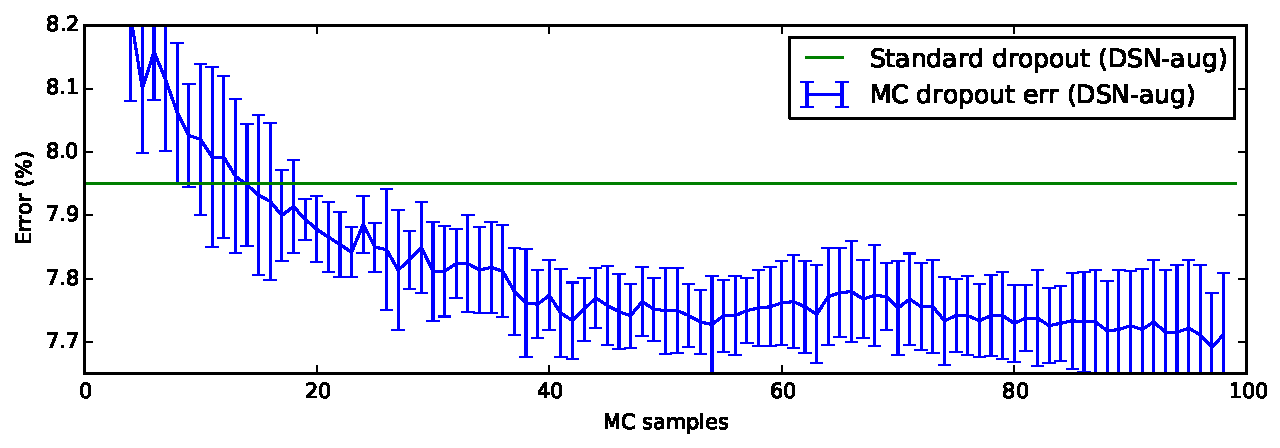
\includegraphics[width=1.0\textwidth]{uncertainty/DSN_samples}
		\caption{Ovisnost klasifikacijske pogreške (plavo) o broju uzoraka u \textit{Monte Carlo} aproksimaciji izlaza na konvolucijskoj mreži koju su ispitivali autori \citep{Gal:2016:BCNNBAVI} na skupu CIFAR-10. Svaka točka je prosjek $5$ mjerenja i prikazane su standardne devijacije. Zeleni pravac označava klasifikacijsku pogrešku kod userdnjavanja kakvo se inače koristi kod testiranja. Slika je preuzeta iz \citet{Gal:2016:BCNNBAVI}.}
		\label{fig:mc-drouput-samples-DSN}
	\end{figure}
\end{frame}


\begin{frame}[allowframebreaks=0.9]{Prepoznavanje izvanrazdiobnih i krivo klasificiranih primjera na temelju izlaza softmaksa ili logita}
\begin{itemize}
	\item Razdiobe koje duboki modeli daju kao izlaz softmaksa su često previše sigurne kod krive klasifikacije i nije ih dobro interpretirati kao vjerojatnosti.
	\item \citet{Hendrycks:2016:BDMOODE} pokazuju da se krivo klasificirani i izvanrazdiobni primjeri ipak mogu uspješno prepoznavati klasifikacijom maksimalne vjerojatnosti softmaksa. 
	\item \citet{Guo:2017:CMNN} pokazuju da se \textbf{temperaturnim skaliranjem} softmaksa može značajno poboljšati kalibracija izlazne razdiobe već naučene mreže. Kod temperaturnog skaliranja, ako su logiti $\vec s$ ($h(\vec x)=\softmax(\vec s)$), izlazni vektor vjerojatnosti uz temperaturno skaliranje je $\softmax\del{\frac{1}{T}\vec s}$.	
	\item \citet{Liang:2017:PDOODENN} predlažu $2$ poboljšanja klasifikacije maksimalne vrijednosti softmaksa za prepoznavanje izvanrazdiobnih primjera. 
	\item Jedno poboljšanje je temperaturno skaliranje. Pokazuju da, što je veća temperatura, to se izvanrazdiobni primjeri mogu bolje odvojiti od unutarrazdiobnih primjera na temelju maksimalne vrijednosti softmaksa. 
	\item Drugo poboljšanje je izmjena ulaza mreže tako da se \textbf{FGSM-om} pomakne u smjeru povećavanja maksimalnog izlaza softmaksa:
	\begin{equation} \label{eq:ODIN-FGSM}
	\tilde{\vec x} = \vec x - \epsilon\sgn\nabla_{\vec x}\del{-\ln \max_k \p(\rvar y=k\mid x,\vec\theta)} \text{.}
	\end{equation}
	$\epsilon$ je parametar koji se određuje pomoću izdvojenog podskupa izvanrazdiobnih primjera.		
	\item Za ovaj rad su još ispitani neki slični pristupi kod kojih se umjesto maksimalnog izlaza softmaksa za prepoznavanje izvanrazdiobnih primjera koristi maksimalni logit ili neke druge značajke izvedene iz vektora logita.
\end{itemize}
\end{frame}


\section{Eksperimenti}

\begin{frame}[allowframebreaks=0.9]{Procjena nesigurnosti kod semantičke segmentacije pomoću dropouta}
\begin{itemize}
	\item Kako bi razlikovali aleatornu i epistemičku nesigurnosti kod semantičke segmentacije, \citet{Kendall:2017:WUNBDLCV} aleatornu nesigurnost modeliraju pomoću predikcije varijanci logita svakog piksela. 
	\item Gubitak za svaki piksel je negativni logaritam vjerojatnosti ciljne klase, a vjerojatnosti se računaju kao očekivanje izlaza softmaksa po razdiobi logita, kao što je opisano jednadžbom~\eqref{eq:kendall-gubitak-klasifikacija}. Očekivanje se procjenjuje \textit{Monte Carlo} aproksimacijom. 
	\item Kao mjeru epistemičke nesigurnosti, \citet{Kendall:2017:WUNBDLCV} za svaki piksel koriste prosječnu varijancu logita uz \textit{MC-dropout}, a aleatornu nesigurnost modeliraju logitima koji imaju Gaussovu razdiobu s dijagonalnom kovarijacijskom matricom, za koju se uči predikcija očekivanja i varijance. 
	\item Ispitan je jednostavniji postupak s procjenom epistemičke nesigurnosti međusobnom informacijom uz \textit{MC-dropout} prema \citet{Rawat:2017:APEBDL,Smith:2018:UMUAED}. 
	
	\item \textit{Monte Carlo} aproksimacija hipoteze je
	\begin{align}
	\overline{h}(\vec x) \coloneqq \frac{1}{M}\sum_{i=1}^M h\del{\vec x;\tilde{\vec\theta}_i} \text{,}
	\end{align}
	gdje je $M$ broj uzoraka, a $\tilde{\vec\theta}_i$ uzorci iz varijacijske razdiobe koja odgovara \textit{dropoutu}.
	\item Procjena ukupne nesigurnosti predikcije je procjena entropije izlazne razdiobe:
	\begin{align} \label{eq:mc-dropout-entropija}
	\H(\rvar y\mid\vec x,\set D)\approx -\overline{h}(\vec x)^\tp\ln\del{\overline{h}(\vec x)} \text{.}
	\end{align}
	\item Aleatorna nesigurnost se procjenjuje kao uvjetna entropija izlazne razdiobe s obzirom na aposteriornu razdiobu parametara prema izrazu~\eqref{eq:mi-aleatorna-nesigurnost}, čemu odgovara aproksimacija prosječnom entropijom uzoraka izlazne razdiobe:
	\begin{align} \label{eq:mc-dropout-aleatorna-nesigurnost}
	\E_{\rvec\theta\mid\set D} \H(\rvar y\mid\vec x,\vec\theta)\approx \frac{1}{M}\sum_{i=1}^M \H\del{\rvec y\midmid\vec x,\rvec\theta=\tilde{\vec\theta}_i} \text{,}
	\end{align}
	gdje je 
	\begin{align}
	\H\del{\rvec y\midmid\vec x,\rvec\theta=\tilde{\vec\theta}_i} = -h\del{\vec x; \tilde{\vec\theta}_i}^\tp\ln\del{h\del{\vec x; \tilde{\vec\theta}_i}}
	\end{align}
	entropija razdiobe izlaza softmaksa $i$-tog uzorka.
	\item Epistemička nesigurnost se procjenjuje kao procjena međusobne informacija prema izrazu~\eqref{eq:mi-epistemicka-nesigurnost}, tj. kao razlika ukupne nesigurnosti u izrazu~\eqref{eq:mc-dropout-entropija} i aleatorne nesigurnosti u izrazu~\eqref{eq:mc-dropout-aleatorna-nesigurnost}:
	\begin{align} \label{eq:mc-dropout-epistemicka nesigurnost}
	\I\del{\del{\rvar y\mid\vec x,\set D};\del{\rvec\theta\mid\set D}} 
	&= \H(\rvar y\mid\vec x,\set D) - \E_{\rvec\theta\mid\set D} \H(\rvar y\mid\vec x,\vec\theta) \\
	&\approx -\overline{h}(\vec x)^\tp\ln\del{\overline{h}(\vec x)} - \frac{1}{M}\sum_{i=1}^M \H\del{\rvec y\midmid\vec x,\rvec\theta=\tilde{\vec\theta}_i} \text{.}
	\end{align}
\end{itemize}
\end{frame}

\begin{frame}[allowframebreaks=0.9]{Procjena nesigurnosti kod semantičke segmentacije pomoću dropouta -- Skupovi podataka}
\begin{itemize}
	\item Za učenje i ispitivanje su korišteni ovi skupovi podataka s oznakama za semantičku segmentaciju:
	\begin{itemize}
		\item CamVid -- skup kojeg čine slijedne slike dimenzija $480\times360$ iz snimki vožnje u gradu s oznakama za $32$ klase. Skup za učenje ima $367$ slika, skup za validaciju $101$, a skup za testiranje $233$.
		\item Cityscapes-- skup slika dimenzija $2048\times1024$ iz vožnje u gradovima s oznakama za $19$ klasa. Skup za učenje ima $2975$ slika, skup za validaciju $500$, a skup za testiranje $1525$ slika.
		\item WildDash -- skup iz vožnje s različitim vremenskim uvjetima, osvjetljenjima, okolinama, vozilima, rijetkim pojavama i s različitim parametrima kamere. Slike su dimenzija $1920\times1080$.
	\end{itemize}
\end{itemize}
\end{frame}

\begin{frame}[allowframebreaks=0.9]{Procjena nesigurnosti kod semantičke segmentacije pomoću dropouta -- Modeli}
\begin{itemize}
	\item Korištena je vlastita implementacija mreže LadderDenseNet-121 \citep{Kreso:2017:LSDFSSLNI} za semantičku segmentaciju. One ne postiže jednako dobru performansu kao originalna. Za dio mreže koji čini DenseNet-121 korištena je inicijalizacija parametrima mreže DenseNet-121 učene na ImageNet-u \citep{Deng:2009:ILSHID}.
	\item Korišten je \textit{dropout} s vjerojatnošću isključivanja $0.2$.
	\item Za \textit{MC-dropout} je kao kod \citet{Kendall:2017:WUNBDLCV} korišteno po $50$ uzoraka za procjenu izlazne razdiobe klasa i nesigurnosti za svaki primjer.	
\end{itemize}
\end{frame}

\begin{frame}[allowframebreaks=0.9]{Procjena nesigurnosti kod semantičke segmentacije pomoću dropouta -- Rezultati}
	\begin{table}
		\centering\small
		\begin{tabular}{lrr}
			\toprule
			\bfseries Model & $\mIoU/\%$ & $A/\%$ \\
			\midrule
			DenseNet + \textit{dropout} \citep{Kendall:2017:WUNBDLCV} & $67.1$ & - \\
			+ aleatorna nesigurnost & $67.2$ & - \\
			+ \textit{MC-dropout} & $67.3$ & -  \\
			+ aleatorna nesigurnost i \textit{MC-dropout} & $67.4$ & -\\
			\midrule
			LadderDenseNet-121-V ($30$ epoha) & $67.7$ & $91.8$ \\
			%		+ \textit{dropout}-$0.1$ & $0.678$ & $0.913$ \\
			%		+ \textit{MC-dropout}-$0.1$ & $0.677$ & $0.915$ \\
			+ \textit{dropout} & $65.8$ & $91.0$ \\
			+ \textit{MC-dropout} & $66.3$ & $91.2$
			\\\bottomrule
		\end{tabular}
		\caption{Usporedba rezultata evaluacije na skupu CamVid. Vrijednosti za LadderDenseNet-121-V bez \textit{dropouta} su prosjek $5$ evaluacija.}
		\label{tab:evaluacija-camvid}
	\end{table}
	
	\begin{table}
		\centering\small
		\begin{tabular}{lrr}
			\toprule
			\bfseries Model & $\mIoU/\%$ & $A/\%$ \\
			\midrule
			LadderDenseNet-121 \citep{Kreso:2017:LSDFSSLNI} & $72.82\phantom{(0.00)}$ & $95.06\phantom{(0.00)}$ \\
			\midrule
			LadderDenseNet-121-V & $67.21(0.70)$ & $94.59(0.06)$ \\
			+ \textit{dropout} & $62.82(0.75)$ & $93.44(0.06)$ \\
			+ \textit{MC-dropout} & $64.16(0.45)$ & $93.90(0.04)$
			\\\bottomrule
		\end{tabular}
		\caption{Usporedba rezultata evaluacije na validacijskom skupu Cityscapesa. Vrijednosti su prosjek $5$ evaluacija. U zagradama su standardne devijacije.}
		\label{tab:evaluacija-cityscapes}
	\end{table}
\begin{itemize}
	\item Napravljeni su eksperimenti s učenjem i ispitivanjem na različitim skupovima.
	\item Još su napravljeni eksperimenti s različitim brojevima epoha i različitim veličinama skupa za učenje s CamVidom. Rezultati tih eksperimenata su prikazani u tablici~\ref{tab:camvid-nesigurnost-epohe-dijelovi-skupa-za-ucenje}.
	\item U tablici~\ref{subtab:camvid-nesigurnost-epohe-dijelovi-skupa-za-ucenje} se vidi da, kako se skupa za učenje smanjuje, aleatorne nesigurnosti raste brže od procjene epistemičke nesigurnosti, što nije u skladu s očekivanjem. 
	\item Još nešto što se može primijetiti u tablici~\ref{subtab:camvid-performansa-epohe-dijelovi-skupa-za-ucenje} je da za $120$ epoha obični \textit{dropout} daje bolje rezultate evaluacije nego \textit{MC-dropout} s $50$ uzoraka.
\end{itemize}
	\begin{table}
		\centering\footnotesize
		\begin{tabular}{llrrrr}
			\toprule
			\bfseries \makecell[l]{Skup za\\ učenje} & \bfseries \makecell[l]{Skup za\\ testiranje} & $\mIoU$ & \bfseries \makecell[r]{Epistemička\\ nesigurnost} & \bfseries \makecell[r]{Aleatorna\\ nesigurnost}  & \makecell[r]{$\frac{\text{epistemička}}{\text{aleatorna}}$} \\
			\midrule
			$\text{CamVid}_\text{trainval}$ & $\text{CamVid}_\text{test}$ & $0.663$ & $0.025$ & $0.207$ & $0.121$ \\
			%$\text{CamVid}_{\text{trainval},1/2}$ & $\text{CamVid}_\text{test}$ & $0.615$ & $0.026$ & $0.272$ & $0.097$ \\
			%$\text{CamVid}_{\text{trainval},1/4}$ & $\text{CamVid}_\text{test}$ & $0.546$ & $0.029$ & $0.391$ & $0.073$ \\
			%$\text{CamVid}_{\text{trainval},1/8}$ & $\text{CamVid}_\text{test}$ & $0.460$ & $0.034$ & $0.538$ & $0.063$ \\
			\midrule
			$\text{CamVid}_\text{trainval}$     & $\text{CamVid}_\text{val}$ & $0.827$ & $0.011$ & $0.118$ & $0.093$ \\
			\midrule
			$\text{CamVid}_\text{trainval}$  & $\text{Cityscapes}_\text{test}$ &      -  & $0.060$ & $0.383$ & $0.156$ \\
			$\text{CamVid}_\text{trainval}$  & 	$\text{WildDash}_\text{bench}$	 &      -  & $0.075$ & $0.501$ & $0.149$ \\
			\midrule
			$\text{Cityscapes}_\text{train}$ & $\text{Cityscapes}_\text{val}$  & $0.644$ & $0.024$ & $0.187$ & $0.126$ \\
			$\text{Cityscapes}_\text{train}$ & $\text{Cityscapes}_\text{test}$ & -       & $0.020$ & $0.162$ & $0.122$ \\
			$\text{Cityscapes}_\text{train}$ & $\text{WildDash}_\text{bench}$  & - & $0.153$ & $0.600$ & $0.254$ \\
			\bottomrule
		\end{tabular}
		\caption{Srednje procjene epistemičke i aleatorne nesigurnosti za različite parove skupa za učenje i skupa za ispitivanje i njihovi omjeri. U indeksima su imena podskupova. $1/n$ u indeksu označava da se uzima slučajan podskup s $1/n$ od svih primjera. Svakom skupu za učenje odgovara jedna mreža.}
		\label{tab:epistemicka-aleatorna-ucenje-testiranje}
	\end{table}
	
	\begin{table}
		\begin{subtable}[t]{1\textwidth}
			\centering
			\begingroup
			\footnotesize
			\newcommand\hnc[1]{\phantom{\mathbf{00.0}}\mathllap{#1}}
			\begin{tabular}{c rrr rrr}
				\toprule
				\bfseries \multirowcell{2}{$\alpha$} & \multicolumn{3}{r}{$\mIoU/\%$} & \multicolumn{3}{r}{$A/\%$} \\
				\cmidrule{2-7}
				{} &$30$ epoha & $60$ epoha & $120$ epoha & $30$ epoha & $60$ epoha & $120$ epoha \\
				\midrule
				$1/1$ 
				& $\hnc{65.6}\;\hnc{66.1}$ &  $\hnc{67.8}\;\hnc{68.0}$ &  $\hnc{68.0}\;\hnc{68.4}$
				& $\hnc{90.9}\;\hnc{91.1}$ &  $\hnc{91.3}\;\hnc{91.5}$ &  $\hnc{91.4}\;\hnc{91.7}$ \\
				$1/2$ 
				& $\hnc{63.2}\;\hnc{63.3}$ &  $\hnc{65.0}\;\hnc{65.5}$ &  $\hnc{66.1}\;\hnc{66.1}$
				& $\hnc{90.2}\;\hnc{90.5}$ &  $\hnc{90.7}\;\hnc{91.0}$ &  $\hnc{90.7}\;\hnc{90.9}$ \\
				$1/4$ 
				& $\hnc{53.4}\;\hnc{55.4}$ &  $\hnc{58.6}\;\hnc{58.8}$ &  $\hnc{60.9}\;\hnc{60.5}$
				& $\hnc{88.3}\;\hnc{89.0}$ &  $\hnc{89.2}\;\hnc{89.6}$ &  $\hnc{89.8}\;\hnc{89.9}$ \\
				$1/8$ 
				& $\hnc{45.1}\;\hnc{46.6}$ &  $\hnc{53.7}\;\hnc{53.2}$ &  $\hnc{56.6}\;\hnc{55.3}$
				& $\hnc{85.1}\;\hnc{86.5}$ &  $\hnc{87.6}\;\hnc{87.7}$ &  $\hnc{88.1}\;\hnc{88.0}$ \\
				\bottomrule
			\end{tabular}			
			\endgroup
			\caption{Srednji omjer presjeka i unije i točnost za \textit{dropout} i \textit{MC-dropout}, ovisno o veličini skupa za učenje i broju epoha. U parovima vrijednosti prva se odnosi na \textit{dropout}, a druga na \textit{MC-dropout}. Svaki par vrijednosti je artimetička sredina evaluacije triju mreža.}
			\label{subtab:camvid-performansa-epohe-dijelovi-skupa-za-ucenje}
		\end{subtable}
		\vskip\baselineskip
		\begin{subtable}[t]{1\textwidth}
			\centering
			\begingroup
			\footnotesize
			\newcommand\hnc[1]{\phantom{\mathbf{0.000}}\mathllap{#1}}
			\begin{tabular}{c rrr}
				\toprule
				$\alpha$ & $30$ epoha & $60$ epoha & $120$ epoha \\
				\midrule
				$1/1$ 
				& $\hnc{0.026}\;\hnc{0.206}\;\hnc{0.128}$ &  $\hnc{0.026}\;\hnc{0.158}\;\hnc{0.164}$ &  $\hnc{0.028}\;\hnc{0.129}\;\hnc{0.213}$
				\\
				$1/2$ 
				& $\hnc{0.044}\;\hnc{0.295}\;\hnc{0.150}$ &  $\hnc{0.028}\;\hnc{0.193}\;\hnc{0.144}$ &  $\hnc{0.029}\;\hnc{0.148}\;\hnc{0.193}$
				\\
				$1/4$ 
				& $\hnc{0.031}\;\hnc{0.397}\;\hnc{0.077}$ &  $\hnc{0.031}\;\hnc{0.272}\;\hnc{0.113}$ &  $\hnc{0.030}\;\hnc{0.181}\;\hnc{0.164}$
				\\
				$1/8$ 
				& $\hnc{0.032}\;\hnc{0.540}\;\hnc{0.059}$ &  $\hnc{0.032}\;\hnc{0.373}\;\hnc{0.085}$ &  $\hnc{0.034}\;\hnc{0.271}\;\hnc{0.125}$
				\\
				\bottomrule
			\end{tabular}			
			\endgroup
			\caption{Prosječna procjena epistemičke nesigurnosti, prosječna procjena aleatorne nesigurnosti i njihov omjer, ovisno o veličini skupa za učenje i broju epoha. Svaka trojka vrijednosti dobivena je jednim mjerenjem.}
			\label{subtab:camvid-nesigurnost-epohe-dijelovi-skupa-za-ucenje}
		\end{subtable}
		\caption{Rezultati evaluacije i prosječne procjene nesigurnosti na skupu za testiranje CamVida. $\alpha$ označava omjer veličine slučajnog podskupa korištenog tijekom učenja i veličine cijelog skupa korištenog za učenje.}
		\label{tab:camvid-nesigurnost-epohe-dijelovi-skupa-za-ucenje}
	\end{table}
\begin{itemize}
	\item Na slikama~\ref{fig:nesigurnost-predikcije-cityscapes}~i~\ref{fig:nesigurnost-predikcije-wilddash} su prikazani odabrani primjeri predikcija i nesigurnosti kod kojih se vidi razlika između procjene aleatorne i procjene epistemičke nesigurnosti. Reci redom predstavljaju:
	\begin{enumerate}
		\item ulaznu sliku
		\item ciljne oznake (samo kod Cityscapesa ako ih ima)
		\item segmentaciju dobivenu običnim \textit{dropoutom}
		\item segmentaciju dobivenu \textit{MC-dropoutom}
		\item entropije izlaznih razdioba po pikselima dobivene običnim \textit{dropoutom}
		\item entropije izlaznih razdioba po pikselima dobivene \textit{MC-dropoutom}
		\item procjenu aleatorne nesigurnosti procjenom uvjetne entropije prema izrazu~\eqref{eq:mc-dropout-aleatorna-nesigurnost} za svaki piksel
		\item procjenu epistemičke nesigurnosti procjenom međusobne informacije prema izrazu~\eqref{eq:mc-dropout-epistemicka nesigurnost} pomnožena s $4$ za svaki piksel.
	\end{enumerate}
	\item Kod slika koje predstavljaju nesigurnost, boje od crne do bijele predstavljaju vrijednosti iz intervala $\intcc{0,\ln C}$, gdje je $C=19$ broj klasa. Jedino za aleatornu nesigurnost, koja je pomnožena s $4$, taj interval je $\intcc{0,\frac{1}{4}\ln C}$ i bijela boja predstavlja sve vrijednosti iz intervala $\intcc{\frac{1}{4}\ln C,\ln C}$. 
	\item Na slici~\ref{fig:boje-klasa-cityscapesa} se vidi koja boja predstavlja koju klasu kod semantičke segmentacije. Mreža je naučena na skupu za učenje Cityscapesa s \textit{dropoutom}.
\end{itemize}
	\begin{figure}
		\centering
		\resizebox{0.61\textwidth}{!}{%
		\begin{minipage}[b]{4.5cm}\offinterlineskip
			\begin{tabu} {@{}X[1,c,m]@{}@{}X[-1,c,m]@{}}
				\makecell[r]{ulaz} & \vspace{1.6cm} \\
				\makecell[r]{ciljna oznaka} & \vspace{1.6cm} \\
				\makecell[r]{predikcija -- \textit{dropout}} & \vspace{1.6cm} \\
				\makecell[r]{predikcija -- \textit{MC-dropout}} &\vspace{1.6cm} \\
				\makecell[r]{entropija -- \textit{dropout}} &\vspace{1.6cm} \\
				\makecell[r]{entropija -- \textit{MC-dropout}} &\vspace{1.6cm} \\
				\makecell[r]{aleatorna nesigurnost} &\vspace{1.6cm} \\
				\makecell[r]{epistemička nesigurnost $\cdot$ $4$ } &\vspace{1.6cm} \\
			\end{tabu}
		\end{minipage}
		\raisebox{-.5\height+0.85mm}{\includegraphics[height=12.8cm,keepaspectratio]{experiments/uncertainty-predictions-cityscapes.png}}
		}		
		\caption{Predikcije i procjene nesigurnosti na odabranim slikama iz skupova za validaciju i testiranje Cityscapesa.}
		\label{fig:nesigurnost-predikcije-cityscapes}
	\end{figure}
	
	\begin{figure}
		\centering
		\resizebox{0.61\textwidth}{!}{%
		\begin{minipage}[b]{4.5cm}\offinterlineskip
			\begin{tabu} {@{}X[1,c,m]@{}@{}X[-1,c,m]@{}}
				\makecell[r]{ulaz} & \vspace{1.6cm} \\
				\makecell[r]{predikcija -- \textit{dropout}} & \vspace{1.6cm} \\
				\makecell[r]{predikcija -- \textit{MC-dropout}} &\vspace{1.6cm} \\
				\makecell[r]{entropija -- \textit{dropout}} &\vspace{1.6cm} \\
				\makecell[r]{entropija -- \textit{MC-dropout}} &\vspace{1.6cm} \\
				\makecell[r]{aleatorna nesigurnost} &\vspace{1.6cm} \\
				\makecell[r]{epistemička nesigurnost $\cdot$ $4$ } &\vspace{1.6cm} \\
			\end{tabu}
		\end{minipage}
		\raisebox{-.5\height+0.85mm}{\includegraphics[height=11.2cm,keepaspectratio]{experiments/uncertainty-predictions-wilddash.png}}
		}
		\caption{Predikcije i procjene nesigurnosti na odabranim slikama iz skupa WildDash.}
		\label{fig:nesigurnost-predikcije-wilddash}
	\end{figure}
	
	\begin{figure}
		\centering
		\resizebox{0.18\textwidth}{!}{%
		\footnotesize
		\begin{minipage}[b]{3.2cm}\offinterlineskip
			\begin{tabu} {@{}X[1,r,m]@{} @{}X[-1,c,m]@{}}
				neoznačeno &\vspace{0.5cm} \\
				cesta &\vspace{0.5cm} \\
				nogostup &\vspace{0.5cm} \\
				građevina &\vspace{0.5cm} \\
				zid &\vspace{0.5cm} \\
				ograda &\vspace{0.5cm} \\
				stup &\vspace{0.5cm} \\
				semafor &\vspace{0.5cm} \\
				prometni~znak &\vspace{0.5cm} \\
				vegetacija &\vspace{0.5cm} \\			
				teren &\vspace{0.5cm} \\			
				nebo &\vspace{0.5cm} \\			
				čovjek &\vspace{0.5cm} \\			
				biciklist ili motociklist &\vspace{0.5cm} \\
				automobil &\vspace{0.5cm} \\
				kamion &\vspace{0.5cm} \\			
				autobus &\vspace{0.5cm} \\			
				vlak &\vspace{0.5cm} \\	
				motocikl &\vspace{0.5cm} \\	
				bicikl &\vspace{0.5cm} \\
			\end{tabu}
		\end{minipage}
		\raisebox{-.5\height+0.85mm}{
\includegraphics[height=10cm,keepaspectratio]{experiments/cityscapes-colors.png}}
		}
		\caption{Nazivi klasa i boje kojima su označene klase Cityscapesa.}
		\label{fig:boje-klasa-cityscapesa}
	\end{figure}

\end{frame}

\section{Prepoznavanje izvanrazdiobnih primjera na temelju izlaza softmaksa ili logita}

\begin{frame}[allowframebreaks=0.9]{Prepoznavanje izvanrazdiobnih primjera na temelju izlaza softmaksa ili logita }
Isprobani su postupci koji su opisani u odjeljku~\ref{subsec:pristupi-ood-softmaks-logiti}, tj. prepoznavanje izvanrazdiobnih primjera na temelju maksimalnog izlaza softmaksa \citep{Hendrycks:2016:BDMOODE} i postupak predložen u \citet{Liang:2017:PDOODENN}. Uz to su isprobani analogni postupci kod kojih se klasifikacija provodi na temelju maksimalnog logita -- klasifikacija na temelju maksmialnog logita uz pomak i bez pomaka ulaza u smjeru povećanja vjerojatnosti klase maksimalnog izlaza softmaksa prema izrazu~\eqref{eq:ODIN-FGSM}.

\end{frame}

\begin{frame}[allowframebreaks=0.9]{Prepoznavanje izvanrazdiobnih primjera na temelju izlaza softmaksa ili logita -- Modeli}

Za ispitivanje su korištene rezidualna mreža WRN-28-10 \citep{Zagoruyko:2016:WRN} i mreža DenseNetBC \citep{Huang:2016:DCCN} s dubinom $L=100$ i faktorom rasta (engl. \textit{growth rate}) $k=12$, koja će biti označavana s \textit{DN-100-12}. Ni kod jedne mreže se ne koristi \textit{dropout}. Korištene su vlastite implementacije tih mreža koje se ne bi trebale previše razlikovati od originalnih, tj. trebalo bi biti sve isto kao što je opisano u \citet{Zagoruyko:2016:WRN,Huang:2016:DCCN}. I jedna i druga ipak postižu malo manju točnost od originalnih mreža na skupu za testiranje skupa CIFAR-10 \citep{Krizhevsky:2009:LMLFTI}. U  tablici~\ref{tab:evaluacija-cifar} su uspoređene performanse mreža korištenih u eksperimentima s performansama originalnih implementacija.

\begin{table}
	\centering\small
	\begin{tabular}{lr}
		\toprule
		\bfseries Model & $A$ \\
		\midrule
		WRN-28-10 \citep{Zagoruyko:2016:WRN} & $0.960$ \\
		DN-100-12 \citep{Huang:2016:DCCN} & $0.955$ \\
		\midrule
		WRN-28-10 & $0.957$ \\
		DN-100-12 & $0.948$ \\
		\bottomrule
	\end{tabular}
	\caption{Usporedba rezultata evaluacije na CIFAR-u s rezultatima autora za mreže korištene u eksperimentima.}
	\label{tab:evaluacija-cifar}
\end{table}
\end{frame}

\begin{frame}[allowframebreaks=0.9]{Prepoznavanje izvanrazdiobnih primjera na temelju izlaza softmaksa ili logita -- Skupovi podataka}
Za ove eksperimente je kao unutarrazdiobni skup korišten podskup za testiranje iz skupa CIFAR-10. CIFAR-10 ima 10 klasa. Slike su dimenzija $32\times 32$ i ima ih $10000$ u skupu za testiranje. Za izvanrazdiobne skupove su, slično kao kod \citet{Hendrycks:2016:BDMOODE,Liang:2017:PDOODENN}, korišteni skupovi:
\begin{enumerate}
	\item TinyImageNet\footnote{\url{https://tiny-imagenet.herokuapp.com/}} --- podskup ImageNet-a \citep{Deng:2009:ILSHID} sa slikama iz $200$ klasa. Skup za testiranje sadrži $10000$ slika. Za ove eksperimente su iz skupa za testiranje konstruirana dva skupa: TinyImageNet-C, koji čine slike iz kojih su nasumično izrezani dijelovi dimenzija $32\times 32$, i TinyImageNet-R, koji čine slike umanjene na iste dimenzije, tj. dimenzije slika iz skupa CIFAR-10.
	\item LSUN \citep{Yu:2015:LSUN} --- skup sličan TinyImageNetu. Skup za testiranje sastoji se od $10000$ slika. Kao i za TinyImageNet, iz skupa za testiranje konstruirana su dva skupa: LSUN-C, koji čine slike iz kojih su nasumično izrezani dijelovi dimenzija $32\times 32$, i LSUN-R, koji čine slike umanjene slike.
	\item iSUN \citep{Xu:2015:TCSWBET} --- podskup SUN-a \citep{Xiao:2016:SUN}. Za eksperimente se koriste sve slike iSUN-a umanjene na dimenzije $32\times 32$.
	\item Gaussov šum --- slučajni uzorci nizova dimenzija $32\times 32\times 3$ tako da svaki element ima nezavisnu vrijednost iz Gaussove razdiobe s očekivanjem $0$ i varijancom $1$.
	\item Uniformni šum --- slučajni uzorci nizova dimenzija $32\times 32\times 3$ tako da svaki element ima nezavisnu vrijednost iz uniformne razdiobe s očekivanjem $0$ i varijancom $1$.
\end{enumerate}
Kao i kod učenja, za svaki skup, slike koje se daju kao ulaz mreži su normalizirane oduzimanjem prosječne vrijednosti i dijeljenjem sa standardnom devijacijom svake komponente (RGB) prema pikselima u skupu za učenje (i validaciju).
\end{frame}

\begin{frame}[allowframebreaks=0.9]{Prepoznavanje izvanrazdiobnih primjera na temelju izlaza softmaksa ili logita -- Evaluacijske mjere}

Kod svih evaluacijskih mjera, osim jedne, kao pozitivna klasa se uzimaju unutarrazdiobni primjeri. Kao kod \citet{Liang:2017:PDOODENN}, koriste se sljedeće evaluacijske mjere:
\begin{enumerate}
	\item Stopa lažnih pozitiva $\FPR$ kada je odziv $0.95$, što će biti označavano $\FPR_{R=0.95}$. $\FPR$ se može interpretirati kao vjerojatnost da se izvanrazdiobni primjer krivo klasificira kao unutarrazdiobni.
	\item $\AUROC$ -- mjera neovisna o pragu i omjeru veličina klasa.
	\item Prosječna preciznost $\AP$ (ili $\AUPR$) -- mjera neovisna o pragu. $\AP$ će označavati prosječnu preciznost kada se unutarrazdiobni ili točno klasificirani primjeri uzimaju kao pozitivna klasa, a $\AP_\text{n}$ kada se izvanrazdiobni ili krivo klasificirani primjeri uzimaju kao pozitivna klasa.
\end{enumerate}

\end{frame}
\begin{frame}[allowframebreaks=0.9]{Procjena nesigurnosti kod semantičke segmentacije pomoću dropouta -- Odabir parametara}

Na temelju rezultata u \citet{Liang:2017:PDOODENN}, koji pokazuju da su veće temperature bolje, za eksperimente u kojima se koristi temperaturno skaliranje softmaksa koristi se temperatura $T=1000$. Za odabir veličine pomaka $\epsilon$ iz svakog izvanrazdiobnog skupa se izvoji $10\%$ slika. Optimalni $\epsilon$ se traži u skupu $\cbr{0,10^{-3},2\cdot 10^{-3},\bidot,12\cdot 10^{-3}}$ tako da minimizira $\FPR$ kad je odziv $0.95$. I kod mreže WRN-28-10 i kod mreže DN-100-12 (vlastitih implementacija), optimalni $\epsilon$ je ispadao otprilike $5$ puta veći nego kod \citet{Liang:2017:PDOODENN} za svaki izvanrazdiobni skup.

\end{frame}

\begin{frame}[allowframebreaks=0.9]{Prepoznavanje izvanrazdiobnih primjera na temelju izlaza softmaksa ili logita -- Rezultati}

Rezultati glavnih eksperimenata su prikazani u tablicama~\ref{tab:ood-dn-cifar}~i~\ref{tab:ood-wrn-cifar}. U tablicama, za svaku evaluacijsku mjeru $5$ stupaca redom predstavlja klasifikaciju po maksimalnoj vrijednosti:
\begin{enumerate}
	\item softmaksa uz $T=1$
	\item softmaksa uz $T=1000$ %(ili logita s pomakom ulaza uz $T\gg 1$)
	\item softmaksa uz $T=1000$ i pomak ulaza FGSM-om
	\item logita
	\item logita uz pomak ulaza FGSM-om.
\end{enumerate}
Kod logita s pomakom ulaza temperatura nije bitna zato što se za pomak ulaza FGSM-om koristi samo predznak gradijenta koji ne ovisi o temperaturi. Neka je $\vec x$ ulaz, $\vec s$ logiti i $\vec y_T \coloneqq \softmax\del{\frac{1}{T}\vec s}$ izlaz softmaksa uz temperaturno skaliranje uz temperaturu $T$. To se može jednostavno pokazati:
\begin{align*}
\sgn\del{ \pd{\vec y_T}{\vec x} }
&= \sgn\del{ \pd{\vec y_T}{\del{\frac{1}{T}\vec s}} \pd{\del{\frac{1}{T}\vec s}}{\vec s} \pd{\vec s}{\vec x}  } 
= \sgn\del{ \pd{\vec y_1}{\del{\vec s}} \del{\frac{1}{T}\cvec I} \pd{\vec s}{\vec x} } \\
&= \sgn\del{ \frac{1}{T} \pd{\vec y_1}{\del{\vec s}} \pd{\vec s}{\vec x}  }
= \sgn\del{ \pd{\vec y_1}{\del{\vec s}} \pd{\vec s}{\vec x}  } 
= \sgn\del{ \pd{\vec y_1}{\vec x}  } \text{.}
\end{align*}

\begin{table} \centering
	\begin{subtable}[t]{1\textwidth}
		\resizebox{\textwidth}{!}{%
			\begingroup
			\newcommand\hnc[1]{\phantom{\mathbf{00.0}}\mathllap{#1}}
			\begin{tabular}{lrrrrr}
				\toprule
				{} &                                                                                 $\mathit{FPR}_{R=0.95}/\%$ &                                                                                        $\mathit{AUROC}/\%$ &                                                               $\mathit{AP}/\%$ &                                                                                $\mathit{AP}_\text{n}/\%$ &                                       $\epsilon/10^{-3}$ \\
				\midrule
				TinyImageNet-C &  $\hnc{51.8}\;\hnc{23.7}\;\hnc{\mathbf{19.0}}\;\hnc{20.8}\;\hnc{\mathbf{19.1}}$ &  $\hnc{92.5}\;\hnc{\mathbf{96.0}}\;\hnc{\mathbf{96.0}}\;\hnc{\mathbf{96.3}}\;\hnc{\mathbf{96.0}}$ &  $\hnc{94.6}\;\hnc{\mathbf{96.8}}\;\hnc{96.4}\;\hnc{\mathbf{96.9}}\;\hnc{96.4}$ &  $\hnc{88.8}\;\hnc{94.7}\;\hnc{\mathbf{95.7}}\;\hnc{\mathbf{95.4}}\;\hnc{\mathbf{95.7}}$ &  $\hnc{0.0}\;\hnc{0.0}\;\hnc{7.0}\;\hnc{0.0}\;\hnc{7.0}$ \\
				TinyImageNet-R &  $\hnc{58.5}\;\hnc{39.5}\;\hnc{\mathbf{36.5}}\;\hnc{37.0}\;\hnc{\mathbf{36.5}}$ &  $\hnc{90.3}\;\hnc{\mathbf{92.4}}\;\hnc{92.3}\;\hnc{\mathbf{92.6}}\;\hnc{92.3}$ &  $\hnc{92.6}\;\hnc{\mathbf{93.6}}\;\hnc{92.9}\;\hnc{\mathbf{93.5}}\;\hnc{92.9}$ &  $\hnc{86.2}\;\hnc{90.6}\;\hnc{\mathbf{91.3}}\;\hnc{\mathbf{91.2}}\;\hnc{\mathbf{91.3}}$ &  $\hnc{0.0}\;\hnc{0.0}\;\hnc{6.0}\;\hnc{0.0}\;\hnc{6.0}$ \\
				LSUN-C         &  $\hnc{54.5}\;\hnc{\mathbf{33.3}}\;\hnc{\mathbf{33.3}}\;\hnc{37.4}\;\hnc{\mathbf{33.3}}$ &  $\hnc{91.7}\;\hnc{\mathbf{94.4}}\;\hnc{\mathbf{94.4}}\;\hnc{93.3}\;\hnc{\mathbf{94.4}}$ &  $\hnc{94.0}\;\hnc{\mathbf{95.5}}\;\hnc{\mathbf{95.5}}\;\hnc{94.5}\;\hnc{\mathbf{95.5}}$ &  $\hnc{87.9}\;\hnc{\mathbf{92.9}}\;\hnc{\mathbf{92.9}}\;\hnc{91.6}\;\hnc{\mathbf{92.9}}$ &  $\hnc{0.0}\;\hnc{0.0}\;\hnc{0.0}\;\hnc{0.0}\;\hnc{0.0}$ \\
				LSUN-R         &  $\hnc{48.7}\;\hnc{18.9}\;\hnc{\mathbf{12.1}}\;\hnc{15.5}\;\hnc{\mathbf{12.1}}$ &  $\hnc{93.1}\;\hnc{96.8}\;\hnc{\mathbf{97.7}}\;\hnc{97.3}\;\hnc{\mathbf{97.7}}$ &  $\hnc{95.1}\;\hnc{97.5}\;\hnc{\mathbf{98.1}}\;\hnc{\mathbf{97.8}}\;\hnc{\mathbf{98.1}}$ &  $\hnc{89.8}\;\hnc{95.9}\;\hnc{\mathbf{97.4}}\;\hnc{96.7}\;\hnc{\mathbf{97.4}}$ &  $\hnc{0.0}\;\hnc{0.0}\;\hnc{7.0}\;\hnc{0.0}\;\hnc{7.0}$ \\
				iSUN           &  $\hnc{51.1}\;\hnc{20.5}\;\hnc{\mathbf{12.7}}\;\hnc{16.1}\;\hnc{\mathbf{12.7}}$ &  $\hnc{92.9}\;\hnc{96.6}\;\hnc{\mathbf{97.6}}\;\hnc{97.2}\;\hnc{\mathbf{97.6}}$ &  $\hnc{95.4}\;\hnc{97.7}\;\hnc{\mathbf{98.2}}\;\hnc{\mathbf{98.0}}\;\hnc{\mathbf{98.2}}$ &  $\hnc{88.3}\;\hnc{95.2}\;\hnc{\mathbf{97.0}}\;\hnc{96.2}\;\hnc{\mathbf{97.0}}$ &  $\hnc{0.0}\;\hnc{0.0}\;\hnc{7.0}\;\hnc{0.0}\;\hnc{7.0}$ \\
				Uniformni šum  &  $\hnc{74.3}\;\hnc{6.1}\;\hnc{\mathbf{0.0}}\;\hnc{\mathbf{0.0}}\;\hnc{\mathbf{0.0}}$ &  $\hnc{93.3}\;\hnc{97.0}\;\hnc{\mathbf{98.9}}\;\hnc{\mathbf{98.7}}\;\hnc{\mathbf{98.9}}$ &  $\hnc{96.2}\;\hnc{98.3}\;\hnc{\mathbf{99.3}}\;\hnc{\mathbf{99.2}}\;\hnc{\mathbf{99.3}}$ &  $\hnc{85.2}\;\hnc{91.2}\;\hnc{\mathbf{96.8}}\;\hnc{96.3}\;\hnc{\mathbf{96.8}}$ &  $\hnc{0.0}\;\hnc{0.0}\;\hnc{2.0}\;\hnc{0.0}\;\hnc{2.0}$ \\
				Gaussiov šum   &  $\hnc{74.3}\;\hnc{6.1}\;\hnc{\mathbf{0.0}}\;\hnc{\mathbf{0.0}}\;\hnc{\mathbf{0.0}}$ &  $\hnc{93.3}\;\hnc{97.0}\;\hnc{\mathbf{98.9}}\;\hnc{\mathbf{98.7}}\;\hnc{\mathbf{98.9}}$ &  $\hnc{96.2}\;\hnc{98.3}\;\hnc{\mathbf{99.3}}\;\hnc{\mathbf{99.2}}\;\hnc{\mathbf{99.3}}$ &  $\hnc{85.2}\;\hnc{91.2}\;\hnc{\mathbf{96.8}}\;\hnc{96.3}\;\hnc{\mathbf{96.8}}$ &  $\hnc{0.0}\;\hnc{0.0}\;\hnc{2.0}\;\hnc{0.0}\;\hnc{2.0}$ \\
				\bottomrule
			\end{tabular}			\endgroup
		}
		\caption{DN-100-12}
		\label{tab:ood-dn-cifar}
	\end{subtable}
	\vskip\baselineskip
	\begin{subtable}[t]{1\textwidth}
		\resizebox{\textwidth}{!}{%
			\begingroup
			\newcommand\hnc[1]{\phantom{\mathbf{00.0}}\mathllap{#1}}
			\begin{tabular}{lrrrrr}
				\toprule
				{} &                                                                                 $\mathit{FPR}_{R=0.95}/\%$ &                                                                                        $\mathit{AUROC}/\%$ &                                                               $\mathit{AP}/\%$ &                                                                                $\mathit{AP}_\text{n}/\%$ &                                       $\epsilon/10^{-3}$ \\
				\midrule
				TinyImageNet-C &  $\hnc{50.0}\;\hnc{34.7}\;\hnc{\mathbf{31.4}}\;\hnc{34.0}\;\hnc{\mathbf{31.4}}$ &  $\hnc{91.0}\;\hnc{\mathbf{93.3}}\;\hnc{\mathbf{93.5}}\;\hnc{92.4}\;\hnc{\mathbf{93.5}}$ &  $\hnc{92.8}\;\hnc{\mathbf{94.3}}\;\hnc{93.9}\;\hnc{92.6}\;\hnc{93.9}$ &  $\hnc{87.9}\;\hnc{92.0}\;\hnc{\mathbf{92.7}}\;\hnc{91.9}\;\hnc{\mathbf{92.7}}$ &  $\hnc{0.0}\;\hnc{0.0}\;\hnc{4.0}\;\hnc{0.0}\;\hnc{4.0}$ \\
				TinyImageNet-R &  $\hnc{55.0}\;\hnc{43.2}\;\hnc{\mathbf{42.7}}\;\hnc{49.2}\;\hnc{\mathbf{42.7}}$ &  $\hnc{89.4}\;\hnc{\mathbf{90.2}}\;\hnc{\mathbf{90.0}}\;\hnc{85.7}\;\hnc{\mathbf{90.0}}$ &  $\hnc{\mathbf{90.3}}\;\hnc{\mathbf{90.1}}\;\hnc{89.6}\;\hnc{84.1}\;\hnc{89.6}$ &  $\hnc{86.0}\;\hnc{\mathbf{88.8}}\;\hnc{\mathbf{88.9}}\;\hnc{85.6}\;\hnc{\mathbf{88.9}}$ &  $\hnc{0.0}\;\hnc{0.0}\;\hnc{1.0}\;\hnc{0.0}\;\hnc{1.0}$ \\
				LSUN-C         &  $\hnc{36.3}\;\hnc{\mathbf{16.5}}\;\hnc{\mathbf{16.5}}\;\hnc{34.3}\;\hnc{\mathbf{16.5}}$ &  $\hnc{94.4}\;\hnc{\mathbf{96.8}}\;\hnc{\mathbf{96.8}}\;\hnc{90.5}\;\hnc{\mathbf{96.8}}$ &  $\hnc{95.8}\;\hnc{\mathbf{97.1}}\;\hnc{\mathbf{97.1}}\;\hnc{89.4}\;\hnc{\mathbf{97.1}}$ &  $\hnc{91.7}\;\hnc{\mathbf{96.1}}\;\hnc{\mathbf{96.1}}\;\hnc{91.1}\;\hnc{\mathbf{96.1}}$ &  $\hnc{0.0}\;\hnc{0.0}\;\hnc{0.0}\;\hnc{0.0}\;\hnc{0.0}$ \\
				LSUN-R         &  $\hnc{47.3}\;\hnc{28.0}\;\hnc{\mathbf{22.3}}\;\hnc{24.2}\;\hnc{\mathbf{22.3}}$ &  $\hnc{92.6}\;\hnc{\mathbf{94.6}}\;\hnc{\mathbf{94.8}}\;\hnc{94.2}\;\hnc{\mathbf{94.8}}$ &  $\hnc{94.2}\;\hnc{\mathbf{95.2}}\;\hnc{94.7}\;\hnc{94.0}\;\hnc{94.7}$ &  $\hnc{89.4}\;\hnc{93.5}\;\hnc{\mathbf{94.6}}\;\hnc{94.1}\;\hnc{\mathbf{94.6}}$ &  $\hnc{0.0}\;\hnc{0.0}\;\hnc{4.0}\;\hnc{0.0}\;\hnc{4.0}$ \\
				iSUN           &  $\hnc{49.0}\;\hnc{31.8}\;\hnc{\mathbf{25.8}}\;\hnc{26.9}\;\hnc{\mathbf{25.8}}$ &  $\hnc{91.8}\;\hnc{93.9}\;\hnc{\mathbf{94.3}}\;\hnc{93.5}\;\hnc{\mathbf{94.3}}$ &  $\hnc{94.0}\;\hnc{\mathbf{95.0}}\;\hnc{\mathbf{94.9}}\;\hnc{93.8}\;\hnc{\mathbf{94.9}}$ &  $\hnc{87.4}\;\hnc{91.9}\;\hnc{\mathbf{93.3}}\;\hnc{92.8}\;\hnc{\mathbf{93.3}}$ &  $\hnc{0.0}\;\hnc{0.0}\;\hnc{3.0}\;\hnc{0.0}\;\hnc{3.0}$ \\
				Uniformni šum  &  $\hnc{88.2}\;\hnc{71.8}\;\hnc{\mathbf{0.0}}\;\hnc{2.1}\;\hnc{\mathbf{0.0}}$ &  $\hnc{87.4}\;\hnc{91.6}\;\hnc{\mathbf{98.7}}\;\hnc{98.3}\;\hnc{\mathbf{98.7}}$ &  $\hnc{92.6}\;\hnc{95.0}\;\hnc{\mathbf{99.1}}\;\hnc{\mathbf{98.9}}\;\hnc{\mathbf{99.1}}$ &  $\hnc{75.1}\;\hnc{82.5}\;\hnc{\mathbf{97.8}}\;\hnc{97.0}\;\hnc{\mathbf{97.8}}$ &  $\hnc{0.0}\;\hnc{0.0}\;\hnc{7.0}\;\hnc{0.0}\;\hnc{7.0}$ \\
				Gaussiov šum   &  $\hnc{88.2}\;\hnc{71.8}\;\hnc{\mathbf{0.0}}\;\hnc{2.1}\;\hnc{\mathbf{0.0}}$ &  $\hnc{87.4}\;\hnc{91.6}\;\hnc{\mathbf{98.7}}\;\hnc{98.3}\;\hnc{\mathbf{98.7}}$ &  $\hnc{92.6}\;\hnc{95.0}\;\hnc{\mathbf{99.1}}\;\hnc{\mathbf{98.9}}\;\hnc{\mathbf{99.1}}$ &  $\hnc{75.1}\;\hnc{82.5}\;\hnc{\mathbf{97.8}}\;\hnc{97.0}\;\hnc{\mathbf{97.8}}$ &  $\hnc{0.0}\;\hnc{0.0}\;\hnc{7.0}\;\hnc{0.0}\;\hnc{7.0}$ \\
				\bottomrule
			\end{tabular}		
			\endgroup
		}
		\caption{WRN-28-10}
		\label{tab:ood-wrn-cifar}
	\end{subtable}
	\caption{Razlikovanje izvanrazdiobnih i unutarrazdiobnih primjera kod mreža naučenih na skupu CIFAR-10. Za svaku evaluacijsku mjeru $5$ stupaca redom predstavlja klasifikaciju po maksimalnoj vrijednosti:	(1) softmaksa uz $T=1$, (2) softmaksa uz $T=1000$, (3) softmaksa uz $T=1000$ i pomak ulaza FGSM-om, (4) logita i (5) logita uz pomak ulaza FGSM-om. Podebljani su najbolji rezultati (više njih ako se razlikuju od najboljeg za manje od $0.003$) za svaki par izvanrazdiobnog skupa i evaluacijske mjere.}
\end{table}

Eksperimenti su pokazali da klasifikacija maksimalnog logita s pomakom ulaza daje skoro jednake rezultate kao klasifikacija maksimalne vrijednosti softmaksa uz $T=1000$, tj. nije se skoro nikad vidjela razlika barem u prve $3$ decimale. Slijedi pokušaj objašnjenja koji ipak ne objašnjava zašto se softmaks s $T=1000$ bez pomaka značajnije razlikuje od logita bez pomaka.
Neka su $s_i=\vec s_\ind{i}$ logiti. Prema definiciji softmaksa,
\begin{align}
\softmax\del{\frac{1}{T}\vec s}_\ind{i} = \frac{\exp(s_i/T)}{\sum_j \exp(s_j/T)} \text{.}
\end{align}
Za dovoljno velik $T$ eksponencijalne funkcije se mogu linearno aproksimirati s malom pogreškom, pa 
\begin{align}
\softmax\del{\frac{1}{T}\vec s}_\ind{i}
\approx \frac{1+s_i/T}{\sum_j (1+s_j/T)}
= \frac{1+s_i/T}{C + \frac{1}{T}\sum_j s_j}
\text{,}
\end{align}
gdje je $C$ broj klasa. U eksperimentima s mrežama naučenim na skupu CIFAR-10, kod mreže DN-100-12 je zbroj logita skoro uvijek u intervalu $\intcc{0.001,0.004}$, a maksimalni logit u intervalu $\intcc{2,30}$, a kod mreže WRN-28-10 je zbroj logita skoro uvijek u intervalu $\intcc{0,0.0004}$, a maksimalni logit u intervalu $\intcc{2,20}$. Primjeri iz različitih skupova su za DN-100-12 prikazani u prostoru \textit{maksimalni~logit~-- zbroj~logita} na slici~\ref{fig:dn-100-12-maxlogits-sumlogits}. Zbrojevi logita podijeljeni s velikom temperaturom $T$, npr. $T=1000$, su zanemarivi u odnosu na $C$ ($C=10$ za CIFAR), pa softmax možemo aproksimirati ovako:
\begin{align}
\softmax\del{\frac{1}{T}\vec s}_\ind{i}
\approx \frac{1+s_i/T}{C}
= \frac{1}{C}+\frac{1}{TC}s_i
\text{.}
\end{align}
Uz ovakvu aproksimaciju vidimo da se maksimalni izlaz softmaksa svodi na afinu transformaciju maksimalnog logita, pa se klasifikacija maksimalne vrijednosti softmaksa svodi na klasifikaciju maksimalnog logita.

\begin{figure}
	\centering
	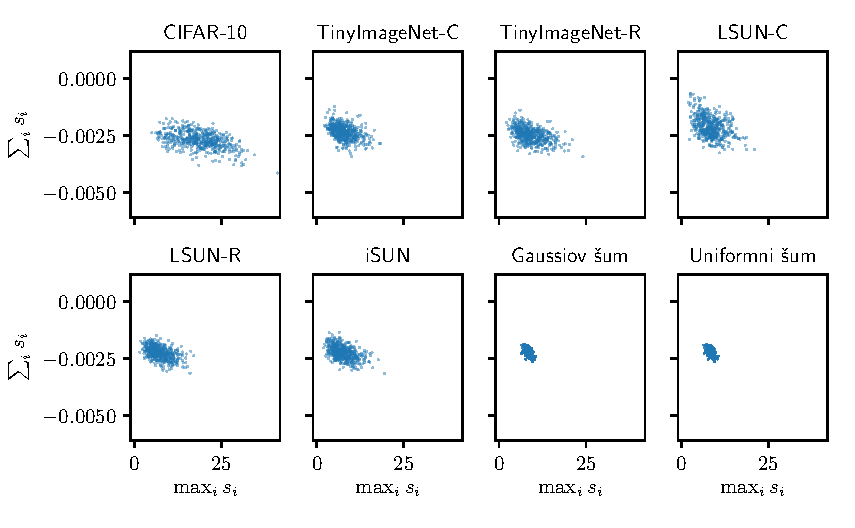
\includegraphics[width=1\textwidth]{dn-100-12-maxlogits-sumlogits}
	\caption{Odnos maksimalnog logita i zbroja logita za različite skupove kod mreže DN-100-12. Svaka točka predstavlja jedan primjer iz podskupova s po $500$ primjera iz skupova korištenih za ispitivanje.}
	\label{fig:dn-100-12-maxlogits-sumlogits}
\end{figure}

U tablici~\ref{tab:krivo-klasificirani-cifar} su prikazani rezultati prepoznavanja krivo klasificiranih primjera. Pozitivna klasa su točno kalsificirani primjeri (njih $9485/10000$ kod DN-100-12 i $9572/10000$ kod WRN-28-10), a negativna klasa su krivo klasificirani primjeri i z skupa CIFAR-10. Kod svih klasifikatora (i kod onih kod kojih nema pomaka ulaza) izdvojeno je oko $10\%$ krivo klasificiranih primjera za odabir veličine	 pomaka $\epsilon$. Vidi se da je ovdje bolja klasifikacija s $T=1$.


\begin{table} \centering
	\resizebox{\textwidth}{!}{%
		\begingroup
		\newcommand\hnc[1]{\phantom{\mathbf{00.0}}\mathllap{#1}}
		\begin{tabular}{llllll}
			\toprule
			{} &                                                                                 $\mathit{FPR}_{R=0.95}/\%$ &                                                                                        $\mathit{AUROC}/\%$ &                                                                                 $\mathit{AP}/\%$ &                                                                                $\mathit{AP}_\text{n}/\%$ &                                       $\epsilon/10^{-3}$ \\
			\midrule
			DN-100-12 &  $\hnc{\mathbf{35.4}}\;\hnc{49.7}\;\hnc{49.7}\;\hnc{49.7}\;\hnc{49.7}$ &  $\hnc{\mathbf{94.2}}\;\hnc{90.4}\;\hnc{90.4}\;\hnc{90.4}\;\hnc{90.4}$ &  $\hnc{\mathbf{99.7}}\;\hnc{\mathbf{99.4}}\;\hnc{\mathbf{99.4}}\;\hnc{\mathbf{99.4}}\;\hnc{\mathbf{99.4}}$ &  $\hnc{\mathbf{45.3}}\;\hnc{35.6}\;\hnc{35.6}\;\hnc{35.6}\;\hnc{35.6}$ &  $\hnc{0.0}\;\hnc{0.0}\;\hnc{0.0}\;\hnc{0.0}\;\hnc{0.0}$ \\
			WRN-28-10 &  $\hnc{\mathbf{34.0}}\;\hnc{37.9}\;\hnc{39.7}\;\hnc{39.2}\;\hnc{39.7}$ &  $\hnc{\mathbf{93.3}}\;\hnc{90.7}\;\hnc{89.6}\;\hnc{89.7}\;\hnc{89.6}$ &  $\hnc{\mathbf{99.7}}\;\hnc{\mathbf{99.5}}\;\hnc{\mathbf{99.4}}\;\hnc{\mathbf{99.4}}\;\hnc{\mathbf{99.4}}$ &  $\hnc{\mathbf{37.5}}\;\hnc{35.9}\;\hnc{34.7}\;\hnc{34.7}\;\hnc{34.6}$ &  $\hnc{0.0}\;\hnc{0.0}\;\hnc{1.0}\;\hnc{0.0}\;\hnc{1.0}$ \\
			\bottomrule
		\end{tabular}			
		\endgroup
	}
	\caption{Prepoznavanje krivo klasificiranih primjera kod mreža naučenih na skupu CIFAR-10. Za svaku evaluacijsku mjeru $5$ stupaca redom predstavlja klasifikaciju po maksimalnoj vrijednosti:	(1) softmaksa uz $T=1$, (2) softmaksa uz $T=1000$, (3) softmaksa uz $T=1000$ i pomak ulaza FGSM-om, (4) logita i (5) logita uz pomak ulaza FGSM-om. Podebljani su najbolji rezultati (više njih ako se razlikuju od najboljeg za manje od $0.003$) za svaku evaluacijsku mjeru.}
	\label{tab:krivo-klasificirani-cifar}
\end{table}
\end{frame}

\begin{frame}[allowframebreaks=0.9]
\frametitle{Literatura}
	\bibliography{literatura}
	\bibliographystyle{fer} 
\end{frame}

\end{document}
